%%%%%%%%%%%%%%%%%%%%%%%%%%%%%%%%%%%%%%%%%%%%%%%%%%%%%%%%%%%%%%%%%%%%%%%%%%%%%%%%%%%%%%%%%%%%%%%%%%%
% Chapter 5 -> Methods
% Author: Mingbo Cheng
%%%%%%%%%%%%%%%%%%%%%%%%%%%%%%%%%%%%%%%%%%%%%%%%%%%%%%%%%%%%%%%%%%%%%%%%%%%%%%%%%%%%%%%%%%%%%%%%%%%
%\addbibresource{~/MEGA/MEGAsync/phd/thesis_Cheng/preamble/thesis.bib}
\chapter{Methods Trajectory Inference}
\label{chapter:methods_TI}
\graphicspath{{chapter5/figs}}

In the previous chapter, we introduced the concept of profiling the single-cell transcriptome, genome, epigenome, and proteome, along with simultaneous sequencing. We also outlined the common workflow for analyzing single-cell sequencing data from different protocols and that of single-cell multimodal analysis. We discussed the challenges associated with single-cell multimodal integration due to various feature distributions and types. To tackle this, our goal is to develop computational methods to effectively integrate single cells of multiple modalities. Another challenge in single-cell multimodal analysis is inferring a trajectory to capture cell fate differentiation. To address this challenge, we aim to develop a computational trajectory inference method tailored for single-cell multimodal data, particularly in complex datasets.

\section{Single cell trajectory inference}
\label{methods:TI}

%a table shows the R dependencies
\subsection{Trajectory Inference}

\begin{algorithm}
    \Input{$A, W, N, \text{pct}, G^{t}=\{\mathcal{V}^{t},\mathcal{E}^{t}\}, K=9$ \Comment{A, W are the Affinity matrix and diffusion distance matrix}
    }
    $i \gets 1$ \\
    $G^{knn}=\{\mathcal{V}^{knn}, \mathcal{E}^{knn}\} \gets \textbf{Graph}(A,W,K)$ \\
    $\mathcal{V}_{low}^{knn} \gets \textbf{LowestPseudotime}(\mathcal{V}^{t}, \text{pct})$ \Comment{pct is percentage parameter}
    $U[v] \gets \textbf{PesudoTime}(v)$ \Comment{Pseudo time of node v}
    $L_p \gets [[]_{1}, []_{2}, \cdots []_{N}]$\\
    \While{$i \leq N$}
    {
        $l_{temp} \gets []$ \\
        $\text{node} \gets \textbf{random}(\mathcal{V}_{low}^{knn})$ \\
        $l_{temp} \gets \textbf{Append}(l_{temp}, \text{node})$ \\
        \While{$\textup{\textbf{true}}$}{
            $\text{NextNodes} \gets \{\mathcal{V} | \mathcal{V}\in \textbf{Neighbor}(\mathcal{E}^{knn}, \text{node}) \text{ and } U[\mathcal{V}]>U[\text{node}]  \}$\\
            \If{$\textup{NextNodes} == \emptyset$}{
                \textbf{break}
            }
            $\text{NextNode} \gets \textbf{PropRandom}(\text{NextNodes})$ \\
            $l_{temp} \gets \textbf{Append}(l_{temp}, \text{NextNode})$ \\
            $\text{node} \gets \text{NextNode}$\\
        }
        $\text{Len} \gets \textbf{Length}(l_{temp})$\\
        $k \gets 1$\\
        \While{$k < \textup{Len}$}{
            $\text{node}_a \gets l_{temp}[k]$\\
            $\text{node}_b \gets l_{temp}[k+1]$\\
            \If{$(\textup{node}_a, \textup{node}_b) \in \mathcal{E}^{t}$}{
                $\text{NodeList} \gets \textbf{ShortestPath}(G^{t}, \text{node}_a, \text{node}_b)$\\
                $L_p[i] \gets \textbf{Append}(L_p[i], \text{node}_a)$\\
                $L_p[i] \gets \textbf{Extend}(L_p[i], \text{NodeList})$\\
            }\Else{
                $L_p[i] \gets \textbf{Append}(L_p[i], \text{node}_a)$\\
            }
        }
        $L_p[i] \gets \textbf{Append}(L_p[i], l_{temp}[\text{Len}])$\\
        $i \gets i+1$\\
    }
    \Return $L_p$
    \caption{Random walk on triangulation graph}
    \label{alg:randomwalk}
\end{algorithm}

\begin{algorithm}
    \KwIn{\\
    $V = \{V_1, V_2,\cdots, V_m\},$ \Comment{cumsum coordinates for each group}
    $t = \{t_1, t_2,\cdots, t_m\},$ \Comment{group pseudo time}
    $min_{bin}=10,$\Comment{shortest trajectory minimum bin size}
    ${\theta}_{cut} = 1,$\Comment{branching point cut distance threshold}
    }
    $t_{min}, t_{max}, R_{max} \gets (\infty, -\infty, -\infty)$\Comment{$R_{max}$ is the maximum range}
    \For{$i\gets1$ \KwTo $m$ \KwBy $1$}{
        $t_{min} \gets \textbf{min}(t_i) \textbf{ if } \textbf{min}(t_i)<t_{min} \textbf{ else } t_{min}$\\
        $t_{max} \gets \textbf{max}(t_i) \textbf{ if } \textbf{min}(t_i)>t_{max} \textbf{ else } t_{max}$\\
        $R_{max} \gets (\textbf{max}({t_i})-\textbf{min}({t_i})) \textbf{ if } (\textbf{max}({t_i})-\textbf{min}({t_i}))>R_{max} \textbf{ else } R_{max}$\\
     }

    $\text{CUTs}, \text{BINs} = [], []$\\
    \For{$i\gets1$ \KwTo $m$ \KwBy $1$}{
        $n_{bin} \gets \lfloor min_{bin} \times \frac{\textbf{max}({t_i}) - \textbf{min}({t_i})}{(t_{max} - t_{min})}\rfloor$\\
        $\text{CUTs}[i] \gets \textbf{linspace}(\textbf{max}({t_i}), \textbf{min}({t_i}), n_{bin}+2)[2:-1]$\\
        $\text{BINs}[i] =[t_i^{1}, t_i^{2}, \cdots t_i^{n_{bin}}]$\\
        $V_i =[V_i^{1}, V_i^{2}, \cdots V_i^{n_{bin}}]$ \Comment{split the $V_{i}$ to be $n_{bin}$}
    }
    $\text{DIC} = \{\}$\Comment{dictionary stores the branching points of all pairs}
    \For{$i\gets1$ \KwTo $m$ \KwBy $1$}{
        %
        \For{$j\gets i+1$ \KwTo $m$ \KwBy $1$ $~\& j \neq i$}{
            $\text{Len}= \textbf{min}(\textbf{length}(V_i), \textbf{length}(V_j))$\\
            \For{$k\gets \textup{Len}$ \KwTo $1$ \KwBy $-1$}{
                $M_i, M_j \gets |\mathbf{V}^k_i|, |\mathbf{V}^k_j|$\\
                $\overline{b^k_i} = \frac{1}{M_i}\sum_{v \in \mathbf{V}^k_i } v$\\
                $\overline{b^k_j} = \frac{1}{M_j}\sum_{v \in \mathbf{V}^k_j } v$\\
                $\overline{\sigma^k_i} = \frac{1}{M_i^2} \sum_{u \in \mathbf{V}^k_i}  \sum_{v \in \mathbf{V}^k_i} \Big\|u-v\Big\|_2$\\
                $\overline{\sigma^k_j} = \frac{1}{M_j^2} \sum_{u \in \mathbf{V}^k_j}  \sum_{v \in \mathbf{V}^k_j} \Big\|u-v\Big\|_2$\\
                $\text{d}(i,j,k) = \Bigg\| \frac{ \overline{b^k_i} }{ \overline{\sigma^k_i}} - \frac{ \overline{b^k_j} }{ \overline{\sigma^k_j}} \Bigg\|_2$\\
                \If{$\text{d}(i,j,k) < {\theta}_{cut}$}{
                    $\text{DIC}(i,j) \gets k$\\
                    $\textbf{break}$\\ 
                }
            }
        }
    }
    
    $\text{invDIC} \gets \textbf{invert}(\text{DIC})$ \Comment{invert dictionary: key,val to val,[key]}
    $\text{bps} \gets \textbf{order}(\textbf{values}(\text{DIC}), \text{ascend}=\text{True})$ \Comment{ordered branching points ids}
    $\text{Tree} = \emptyset$\\
    \While{$\text{bp} \textbf{ in } \text{bps}$}{
        $\text{Tree} \gets \textbf{MergeBranch}(\text{invDIC}, \text{bp})$\Comment{create tree with branching points}
    }

    \Return $\text{Tree}$
    \caption{Tree Creating Algorithm}
    \label{alg:treecreating}
\end{algorithm}

\begin{figure}[!ht]
	\centering
	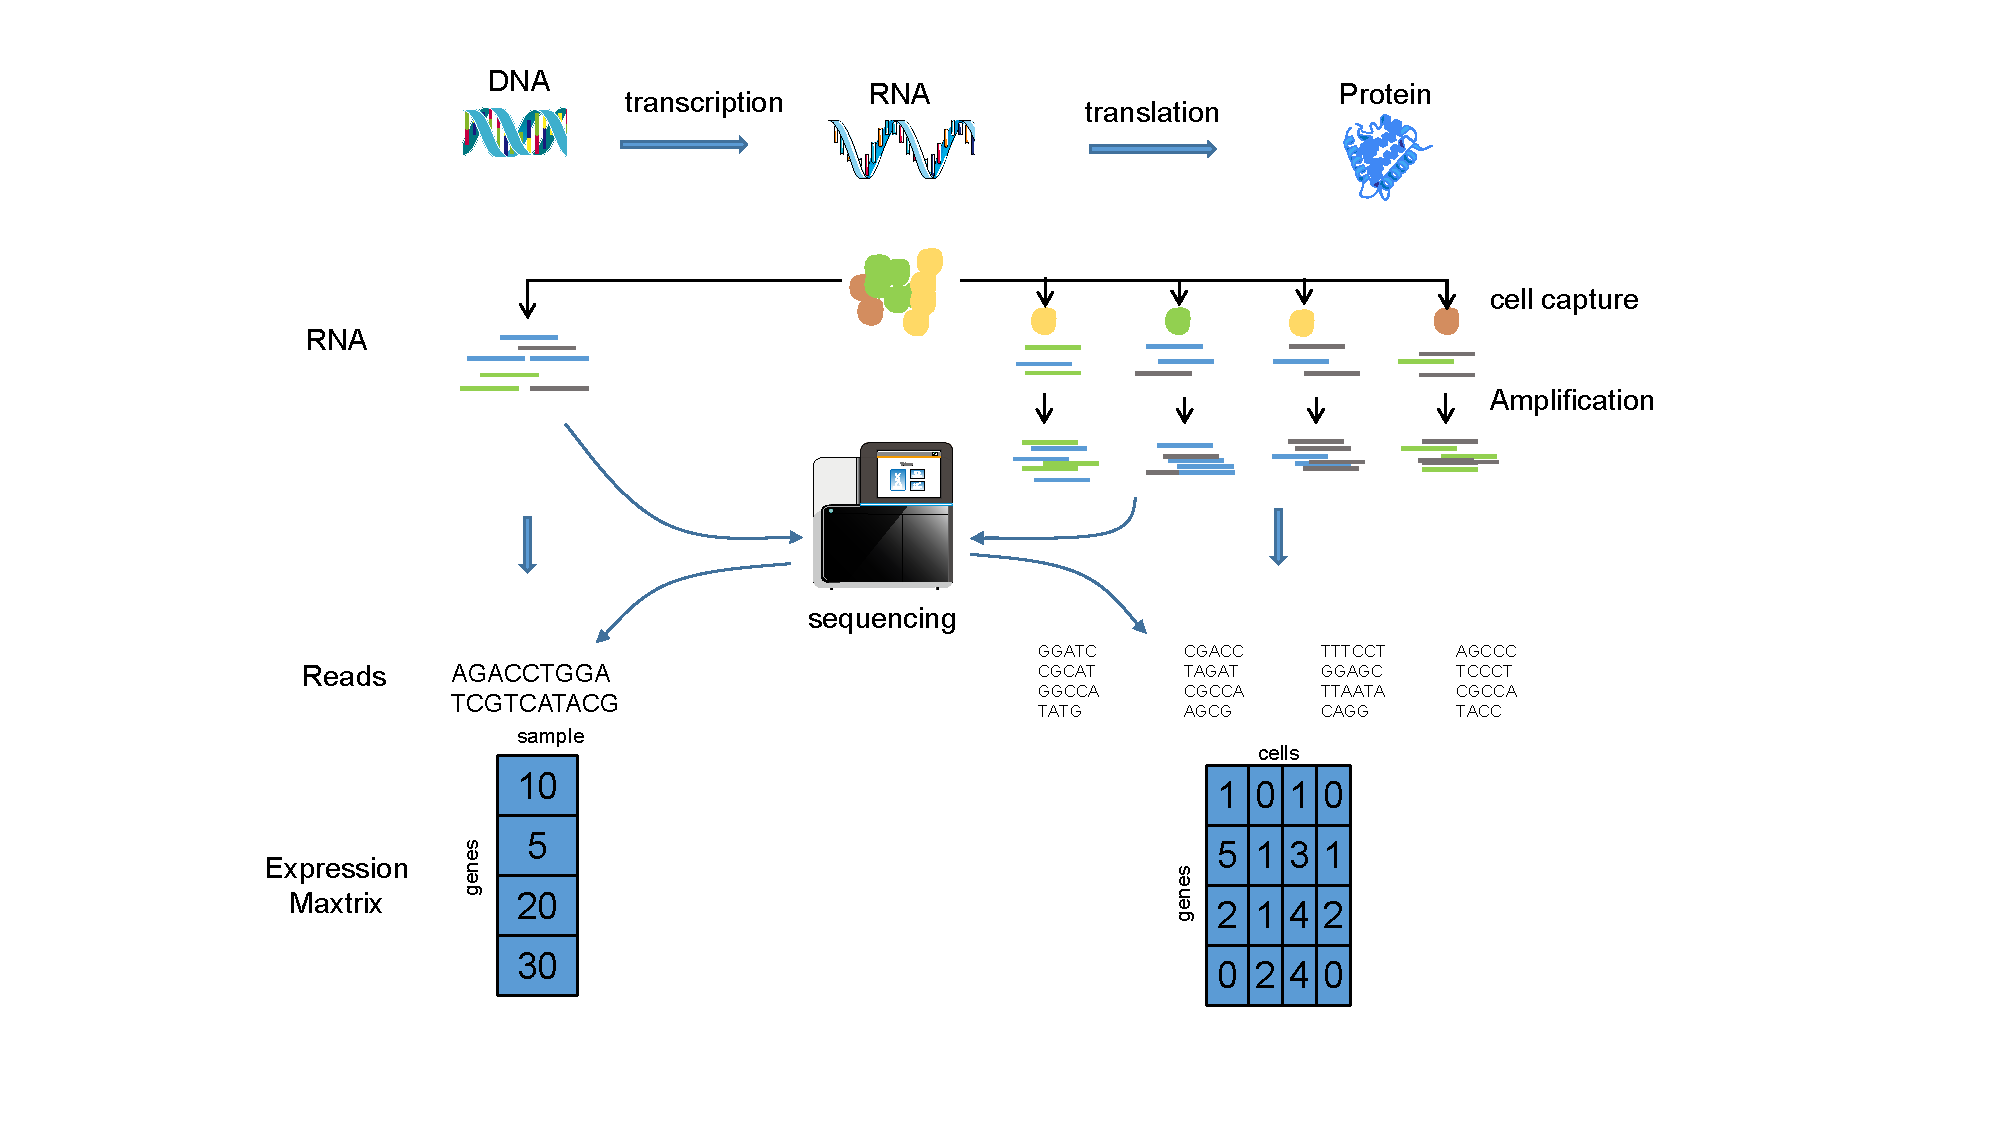
\includegraphics[width=0.95\textwidth]{PHLOWER_schematic/fig}
	\vspace{0.1cm}
	\caption[PHLOWER\_schematic.]{PHLOWER\_schematic}
	\label{fig:PHLOWER_schematic}
\end{figure}

% python package dependencies
\begin{table}[!ht]
	\centering
	\begin{tabular}{lll}
		\toprule
		\textbf{Package} & \textbf{Version} & \textbf{Website} \\
		\midrule
			Numpy& >=1.23.5 & \url{https://numpy.org/} \\
			Matplotlib& >=3.6.0 & \url{https://matplotlib.org/} \\
			Seaborn& >=0.12.0 & \url{https://seaborn.pydata.org/} \\
			Pydot& >=1.4.2 & \url{https://github.com/pydot/pydot} \\
			Igraph& >=0.10.5 & \url{https://igraph.org/python/} \\
			Scikit-learn& >=1.1.2 & \url{https://scikit-learn.org/stable/} \\
			Scipy& >=1.10.1 & \url{https://www.scipy.org/} \\
			Pandas& >=1.3.5 & \url{https://pandas.pydata.org/} \\
			Plotly& >=5.13.1 & \url{https://plotly.com/} \\
			Tqdm& >=4.64.1 & \url{https://github.com/tqdm/tqdm} \\
			Leidenalg& >=0.9.1 & \url{https://github.com/vtraag/leidenalg} \\
			%louvain& >=0.8.0 & \url{} \\
			Colorcet& >=3.0.1 & \url{https://github.com/holoviz/colorcet} \\
			Umap-learn& >=0.5.3 & \url{https://github.com/lmcinnes/umap} \\
			Scikit-sparse& >=0.4.8 & \url{https://github.com/scikit-sparse/scikit-sparse} \\
			Scanpy& >=1.9.3 & \url{https://github.com/scverse/scanpy} \\
			Anndata& >=0.8.0 & \url{https://github.com/scverse/anndata} \\
            Magic-impute & >=0.8.03.0.0 & \url{https://github.com/KrishnaswamyLab/MAGIC}\\
		\bottomrule
	\end{tabular}
	\vspace{0.1cm}
	\caption[PHLOWER tool python package dependencies]{PHLOWER tool python package dependencies.}
	\label{tab:phlower_python_dependencies}
\end{table}
% a table shows the python dependencies
% check how to rotate the title text of a table, see Li's table 3.2

\subsection{Implementation}
We developed our Graph Hodge Laplacian (HL)-based approach to address the trajectory inference (TI) of single-cell multimodal data as a Python module. Our method is named PHLOWER (\textit{gra}\textbf{P}h \textbf{H}odge \textbf{L}aplacian inferring traject\textbf{O}ry flo\textbf{W}s of c\textbf{E}ll diffe\textbf{R}entiation) and will be referred to as such throughout this thesis. The method's implementation encompasses all the steps described in this chapter. PHLOWER was initially released in September 2023. \fref{fig:PHLOWER_schematic} illustrates the workflow of PHLOWER, and \tref{tab:phlower_python_dependencies} summarizes the dependencies of the PHLOWER module.

PHLOWER requires, at a minimum, dimensional reduction as input as well as a count matrix to be processed by itself. The output of PHLOWER is a STREAM tree as visualization that shows the cell differentiation tree. In addition, PHLOWER outputs a tree structure with detailed random walk paths for downstream analysis.

By default, PHLOWER is designed to work seamlessly with Scanpy and Episcanpy. It also offers a range of analysis methods for cell differentiation downstream. For example, `phlower.tl.tree\_mbranch\_markers' is used to find significant markers for each branch against the rest of the branches. Moreover, for multimodal data, such as single-cell transcriptome and open chromatin, one can call `phlower.tl.branch\_TF\_gene\_correlation' to correlate two features along tree branches. With this, one can create a heatmap matrix using the function `phlower.tl.branch\_heatmap\_matrix' to show the features along the trajectories.

To ensure users utilize PHLOWER correctly, we have deployed PHLOWER documents to \url{https://phlower.readthedocs.io/en/latest/}, where one can easily check the vignette for using PHLOWER, as well as the API.

We have tested PHLOWER with Python (3.8-3.10) and required dependencies, such as Numpy 1.23.5, Matplotlib 3.8.1, Seaborn 0.13.0, Pydot 1.4.2, Igraph 0.10.5, Scikit-learn 1.1.2, Scipy 1.10.1, Pandas 2.0.3, Plotly 5.13.1, Tqdm 4.64.1, Leidenalg 0.9.1, Louvain 0.8.0, Colorcet 3.0.1, Umap-learn 0.5.3, Scikit-sparse 0.4.8, Episcanpy 0.4.0, Scanpy 1.9.3, Anndata 0.9.2, Magic-impute 3.0.0.

We executed PHLOWER on a local Linux Mint 21.1 x86\_64 64-bit machine with 12 Intel(R) Core(TM) i5-10400 CPUs at 2.90GHz and 64 GB RAM. Additionally, we ran PHLOWER on a High-Performance Computing (HPC) cluster primarily based on AMD EPYC 7452 64-bit nodes at 2.35 GHz and 500 GB RAM with Rocky Linux 8.9.

For more information about PHLOWER implementation, source code, tutorials and examples, please see:
\begin{center}
\url{https://github.com/CostaLab/phlower}
\end{center}

\subsection{Discussion}
In this section, we discussed our computational methods for single-cell multimodal trajectory inference. We first introduce, next xxx
Finally, we described the implementation details(sref{})

From a conceptual standpoint, when comparing our method of Hodge Laplacian decomposition with competing methods, it becomes evident that the latter either connect clusters to derive trajectories or identify backbones in low dimensions (2,3) to represent trajectories. However, none of these methods effectively utilizes the high dimensions of a graph for inference. In contrast, our method utilizes edges in the high-dimensional cumulative trajectory space to identify branching points. This marks the first time Hodge Laplacian decomposition is employed to create a tree structure. Such innovation can find applications not only in biology but also in areas such as traffic detection and beyond.

\begin{itemize}

    \item We emphasized the utilization of high-level graph information, specifically the Hodge Laplacian, to capture not only relations between vertices and edges but also relations between edges and triangles. Leveraging more information allows us to derive more accurate trajectories for single-cell analysis.

    \item Subsequently, we developed a trajectory inference method based on the decomposition of the Hodge Laplacian. Our approach goes beyond a simple application of this theory to the single-cell trajectory inference problem. Incorporating essential elements such as hole creation and triangulation tricks, we address the nuances of the problem. Additionally, to overcome the issue of preference random walk getting stuck in local areas, we propose a two-step process. First, we perform the walk on the diffusion graph, followed by finding the shortest paths on the triangulated graph. The creation of a tree structure is also crucial, and we achieve this by calculating normalized distances for edges in the cumulative trajectory space to determine branching points

\end{itemize}


\section{Discussion}
In this section, we introduced two frameworks, MOJITOO and PHLOWER, addressing two key challenges in single-cell multimodal analysis: integration analysis and trajectory inference. MOJITOO, an integration method, employs Canonical Correlation Analysis (CCA) to effectively derive a unified latent space from diverse feature matrices. On the other hand, the trajectory inference method, PHLOWER, utilizes the decomposition of the Hodge Laplacian to cluster trajectories and subsequently constructs a cell fate tree to depict the biological cell differentiation process.
